\documentclass[12pt]{article}
\usepackage[]{graphicx}
\usepackage[]{color}
%% maxwidth is the original width if it is less than linewidth
%% otherwise use linewidth (to make sure the graphics do not exceed the margin)
\makeatletter
\def\maxwidth{ %
  \ifdim\Gin@nat@width>\linewidth
    \linewidth
  \else
    \Gin@nat@width
  \fi
}
\makeatother

\definecolor{fgcolor}{rgb}{0.345, 0.345, 0.345}
\newcommand{\hlnum}[1]{\textcolor[rgb]{0.686,0.059,0.569}{#1}}%
\newcommand{\hlstr}[1]{\textcolor[rgb]{0.192,0.494,0.8}{#1}}%
\newcommand{\hlcom}[1]{\textcolor[rgb]{0.678,0.584,0.686}{\textit{#1}}}%
\newcommand{\hlopt}[1]{\textcolor[rgb]{0,0,0}{#1}}%
\newcommand{\hlstd}[1]{\textcolor[rgb]{0.345,0.345,0.345}{#1}}%
\newcommand{\hlkwa}[1]{\textcolor[rgb]{0.161,0.373,0.58}{\textbf{#1}}}%
\newcommand{\hlkwb}[1]{\textcolor[rgb]{0.69,0.353,0.396}{#1}}%
\newcommand{\hlkwc}[1]{\textcolor[rgb]{0.333,0.667,0.333}{#1}}%
\newcommand{\hlkwd}[1]{\textcolor[rgb]{0.737,0.353,0.396}{\textbf{#1}}}%

\usepackage{framed}
\makeatletter
\newenvironment{kframe}{%
 \def\at@end@of@kframe{}%
 \ifinner\ifhmode%
  \def\at@end@of@kframe{\end{minipage}}%
  \begin{minipage}{\columnwidth}%
 \fi\fi%
 \def\FrameCommand##1{\hskip\@totalleftmargin \hskip-\fboxsep
 \colorbox{shadecolor}{##1}\hskip-\fboxsep
     % There is no \\@totalrightmargin, so:
     \hskip-\linewidth \hskip-\@totalleftmargin \hskip\columnwidth}%
 \MakeFramed {\advance\hsize-\width
   \@totalleftmargin\z@ \linewidth\hsize
   \@setminipage}}%
 {\par\unskip\endMakeFramed%
 \at@end@of@kframe}
\makeatother

\definecolor{shadecolor}{rgb}{.97, .97, .97}
\definecolor{messagecolor}{rgb}{0, 0, 0}
\definecolor{warningcolor}{rgb}{1, 0, 1}
\definecolor{errorcolor}{rgb}{1, 0, 0}
\newenvironment{knitrout}{}{} % an empty environment to be redefined in TeX

\usepackage{alltt}

\usepackage{times}
\usepackage{hyperref}
\hypersetup{pdfpagemode=UseNone} % don't show bookmarks on initial view
\hypersetup{colorlinks, urlcolor={blue}}

% revise margins
\setlength{\headheight}{0.0in}
\setlength{\topmargin}{0.0in}
\setlength{\headsep}{0.0in}
\setlength{\textheight}{8.65in}
\setlength{\footskip}{0.35in}
\setlength{\oddsidemargin}{0.0in}
\setlength{\evensidemargin}{0.0in}
\setlength{\textwidth}{6.5in}

\setlength{\parskip}{6pt}
\setlength{\parindent}{0pt}
\IfFileExists{upquote.sty}{\usepackage{upquote}}{}
\begin{document}

{\sffamily \textbf{An example Knitr/R Markdown document}}

\href{http://kbroman.org}{Karl W Broman}

This is a portion of the ``\href{http://www.rqtl.org/rqtltour2.pdf}{A shorter tour of R/qtl}''
tutorial, developed here in multiple formats to illustrate the use of knitr.
This particular document is written with \href{http://www.latex-project.org}{LaTeX}.



\bigskip
{\sffamily \textbf{Preliminaries}}
\nopagebreak

To install R/qtl, you need to first install the package.
Type (within R) {\tt install.packages("qtl")}
(This needs to be done just once.)

You then load the R/qtl package using the {\tt library} function:

\begin{knitrout}
\definecolor{shadecolor}{rgb}{0.969, 0.969, 0.969}\color{fgcolor}\begin{kframe}
\begin{alltt}
\hlkwd{library}\hlstd{(qtl)}
\end{alltt}
\end{kframe}
\end{knitrout}

This needs to be done every time you start R. (There is a way to
have the package loaded automatically every time, but we won't discuss
that here.)

To get help on the functions and data sets in R
(and in R/qtl), use {\tt help()} or {\tt ?}. For example, to view the help
file for the {\tt read.cross} function, type one of the following:

\begin{knitrout}
\definecolor{shadecolor}{rgb}{0.969, 0.969, 0.969}\color{fgcolor}\begin{kframe}
\begin{alltt}
\hlkwd{help}\hlstd{(read.cross)}
\hlopt{?}\hlstd{read.cross}
\end{alltt}
\end{kframe}
\end{knitrout}

\bigskip
{\sffamily \textbf{Data import}}
\nopagebreak

We will consider data from
\href{http://www.ncbi.nlm.nih.gov/pubmed/12118100}{Sugiyama et al.,
Physiol Genomics 10:5--12, 2002}. Load the data into R/qtl as
follows.

\begin{knitrout}
\definecolor{shadecolor}{rgb}{0.969, 0.969, 0.969}\color{fgcolor}\begin{kframe}
\begin{alltt}
\hlstd{sug} \hlkwb{<-} \hlkwd{read.cross}\hlstd{(}\hlstr{"csv"}\hlstd{,} \hlstr{"http://www.rqtl.org"}\hlstd{,} \hlstr{"sug.csv"}\hlstd{,}
                  \hlkwc{genotypes}\hlstd{=}\hlkwd{c}\hlstd{(}\hlstr{"CC"}\hlstd{,} \hlstr{"CB"}\hlstd{,} \hlstr{"BB"}\hlstd{),}
                  \hlkwc{alleles}\hlstd{=}\hlkwd{c}\hlstd{(}\hlstr{"C"}\hlstd{,} \hlstr{"B"}\hlstd{))}
\end{alltt}
\begin{verbatim}
##  --Read the following data:
## 	 163  individuals
## 	 93  markers
## 	 6  phenotypes
##  --Cross type: f2
\end{verbatim}
\end{kframe}
\end{knitrout}


The function {\tt read.cross} is for importing data into R/qtl.
{\tt "sug.csv"} is the name of the file, which we import directly
from the R/qtl website.  {\tt genotypes} indicates the codes used for
the genotypes; {\tt alleles} indicates single-character codes to be
used in plots and such.

{\tt read.cross} loads the data from the file and formats it into
a special cross object, which is then assigned to {\tt sug} via the
assignment operator {\tt <-}.

The data are from an intercross between BALB/cJ and CBA/CaJ; only male
offspring were considered.  There are four phenotypes: blood pressure,
heart rate, body weight, and heart weight.  We will focus on the blood
pressure phenotype, will consider just the 163 individuals with
genotype data and, for simplicity, will focus on the autosomes.


\bigskip
{\sffamily \textbf{Summaries}}
\nopagebreak

The data object {\tt sug} is complex; it contains the genotype
data, phenotype data and genetic map.  R has a certain amount of
``object oriented'' facilities, so that calls to functions like
{\tt summary} and {\tt plot} are interpreted appropriately for the object
considered.

The object {\tt sug} has ``class'' {\tt "cross"}, and so calls to
{\tt summary} and {\tt plot} are actually sent to the functions
{\tt summary.cross} and {\tt plot.cross}.

Use {\tt summary()} to get a quick summary of the data.  (This also
performs a variety of checks of the integrity of the data.)

\begin{knitrout}
\definecolor{shadecolor}{rgb}{0.969, 0.969, 0.969}\color{fgcolor}\begin{kframe}
\begin{alltt}
\hlkwd{summary}\hlstd{(sug)}
\end{alltt}
\begin{verbatim}
##     F2 intercross
## 
##     No. individuals:    163 
## 
##     No. phenotypes:     6 
##     Percent phenotyped: 95.1 95.7 99.4 99.4 100 100 
## 
##     No. chromosomes:    19 
##         Autosomes:      1 2 3 4 5 6 7 8 9 10 11 12 13 14 15 
##                         16 17 18 19 
## 
##     Total markers:      93 
##     No. markers:        5 7 5 5 5 4 8 4 4 5 6 3 3 5 5 4 4 6 
##                         5 
##     Percent genotyped:  98.3 
##     Genotypes (%):      CC:23.9  CB:50.2  BB:26.0 
##                         not BB:0.0  not CC:0.0
\end{verbatim}
\end{kframe}
\end{knitrout}

We see that this is an intercross with 163 individuals.
There are 6 phenotypes, and genotype data at
93 markers across the 19 autosomes.  The genotype
data is quite complete.

Use {\tt plot()} to get a summary plot of the data.

\begin{knitrout}
\definecolor{shadecolor}{rgb}{0.969, 0.969, 0.969}\color{fgcolor}\begin{kframe}
\begin{alltt}
\hlkwd{plot}\hlstd{(sug)}
\end{alltt}
\end{kframe}
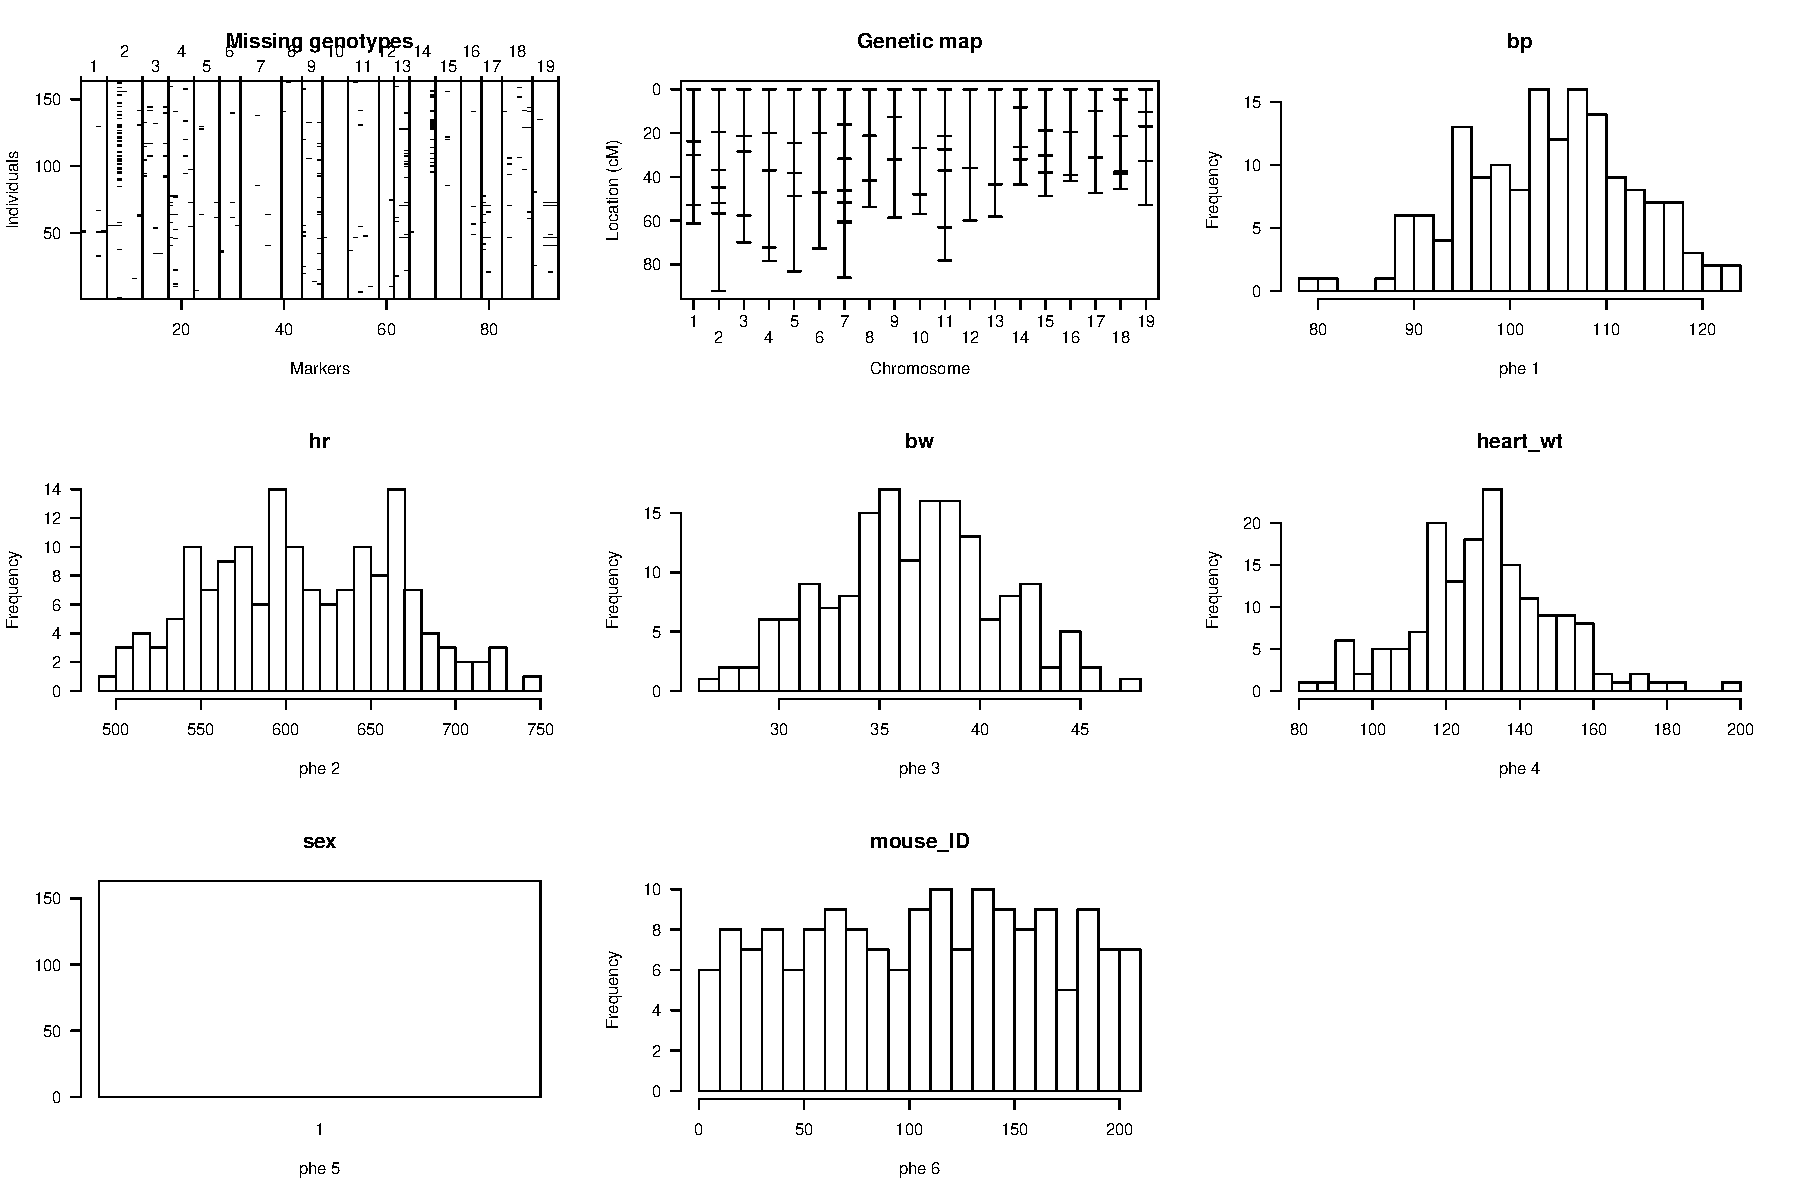
\includegraphics[width=\maxwidth]{RnwFigs/summary_plot-1} 

\end{knitrout}

The plot in the upper-left shows the pattern of missing genotype data, with
black pixels corresponding to missing genotypes.  The next plot shows
the genetic map of the typed markers.  The following plots are
histograms or bar plots for the six phenotypes.  The last two
``phenotypes'' are sex (with 1 corresponding to males) and mouse ID.


\bigskip
{\sffamily \textbf{Single-QTL analysis}}
\nopagebreak

Let's now proceed to QTL mapping via a single-QTL model.

We first calculate the QTL genotype probabilities, given the
observed marker data, via the function {\tt calc.genoprob}.  This is
done at the markers and at a grid along the chromosomes.  The argument
{\tt step} is the density of the grid (in cM), and defines the
density of later QTL analyses.

\begin{knitrout}
\definecolor{shadecolor}{rgb}{0.969, 0.969, 0.969}\color{fgcolor}\begin{kframe}
\begin{alltt}
\hlstd{sug} \hlkwb{<-} \hlkwd{calc.genoprob}\hlstd{(sug,} \hlkwc{step}\hlstd{=}\hlnum{1}\hlstd{)}
\end{alltt}
\end{kframe}
\end{knitrout}

The output of {\tt calc.genoprob} is the same cross object as input,
with additional information (the QTL genotype probabilities) inserted.  We
assign this back to the original object (writing over the previous
data), though it could have also been assigned to a new object.

To perform a single-QTL genome scan, we use the function {\tt scanone}.
By default, it performs standard interval mapping (that is, maximum
likelihood via the EM algorithm).  Also, by default, it considers the
first phenotype in the input cross object (in this case, blood
pressure).

\begin{knitrout}
\definecolor{shadecolor}{rgb}{0.969, 0.969, 0.969}\color{fgcolor}\begin{kframe}
\begin{alltt}
\hlstd{out.em} \hlkwb{<-} \hlkwd{scanone}\hlstd{(sug)}
\end{alltt}
\end{kframe}
\end{knitrout}

The output has ``class'' {\tt "scanone"}.  The {\tt summary}
function is passed to the function {\tt summary.scanone}, and gives
the maximum LOD score on each chromosome.

\begin{knitrout}
\definecolor{shadecolor}{rgb}{0.969, 0.969, 0.969}\color{fgcolor}\begin{kframe}
\begin{alltt}
\hlkwd{summary}\hlstd{(out.em)}
\end{alltt}
\begin{verbatim}
##           chr   pos   lod
## D1MIT36     1 76.73 1.449
## c2.loc77    2 82.80 1.901
## c3.loc42    3 52.82 1.393
## c4.loc43    4 47.23 0.795
## D5MIT223    5 86.57 1.312
## c6.loc26    6 27.81 0.638
## c7.loc45    7 47.71 6.109
## c8.loc34    8 54.90 1.598
## D9MIT71     9 27.07 0.769
## c10.loc51  10 60.75 0.959
## c11.loc34  11 38.70 2.157
## D12MIT145  12  2.23 1.472
## c13.loc20  13 27.26 1.119
## D14MIT138  14 12.52 1.119
## c15.loc8   15 11.96 5.257
## c16.loc31  16 45.69 0.647
## D17MIT16   17 17.98 1.241
## D18MIT22   18 13.41 1.739
## D19MIT71   19 56.28 0.402
\end{verbatim}
\end{kframe}
\end{knitrout}

Alternatively, we can give a threshold, e.g., to only see those
chromosomes with LOD $>$ 3.

\begin{knitrout}
\definecolor{shadecolor}{rgb}{0.969, 0.969, 0.969}\color{fgcolor}\begin{kframe}
\begin{alltt}
\hlkwd{summary}\hlstd{(out.em,} \hlkwc{threshold}\hlstd{=}\hlnum{3}\hlstd{)}
\end{alltt}
\begin{verbatim}
##          chr  pos  lod
## c7.loc45   7 47.7 6.11
## c15.loc8  15 12.0 5.26
\end{verbatim}
\end{kframe}
\end{knitrout}

We can plot the results as follows.

\begin{knitrout}
\definecolor{shadecolor}{rgb}{0.969, 0.969, 0.969}\color{fgcolor}\begin{kframe}
\begin{alltt}
\hlkwd{plot}\hlstd{(out.em)}
\end{alltt}
\end{kframe}
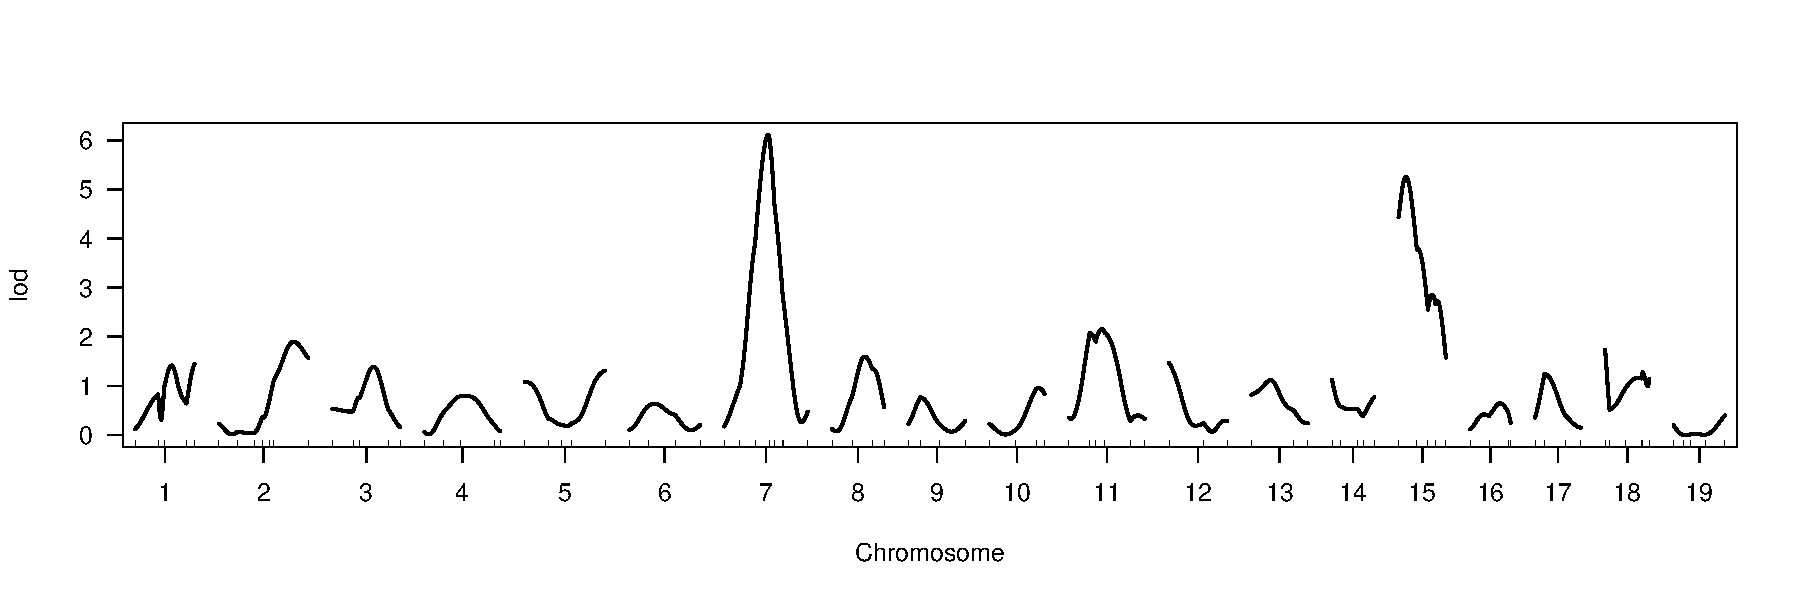
\includegraphics[width=\maxwidth]{RnwFigs/plot_scanone-1} 

\end{knitrout}

We can do the genome scan via Haley-Knott regression by calling
{\tt scanone} with the argument {\tt method="hk"}.

\begin{knitrout}
\definecolor{shadecolor}{rgb}{0.969, 0.969, 0.969}\color{fgcolor}\begin{kframe}
\begin{alltt}
\hlstd{out.hk} \hlkwb{<-} \hlkwd{scanone}\hlstd{(sug,} \hlkwc{method}\hlstd{=}\hlstr{"hk"}\hlstd{)}
\end{alltt}
\end{kframe}
\end{knitrout}

We may plot the two sets of LOD curves together in a single call
to {\tt plot}.

\begin{knitrout}
\definecolor{shadecolor}{rgb}{0.969, 0.969, 0.969}\color{fgcolor}\begin{kframe}
\begin{alltt}
\hlkwd{plot}\hlstd{(out.em, out.hk,} \hlkwc{col}\hlstd{=}\hlkwd{c}\hlstd{(}\hlstr{"blue"}\hlstd{,} \hlstr{"red"}\hlstd{))}
\end{alltt}
\end{kframe}
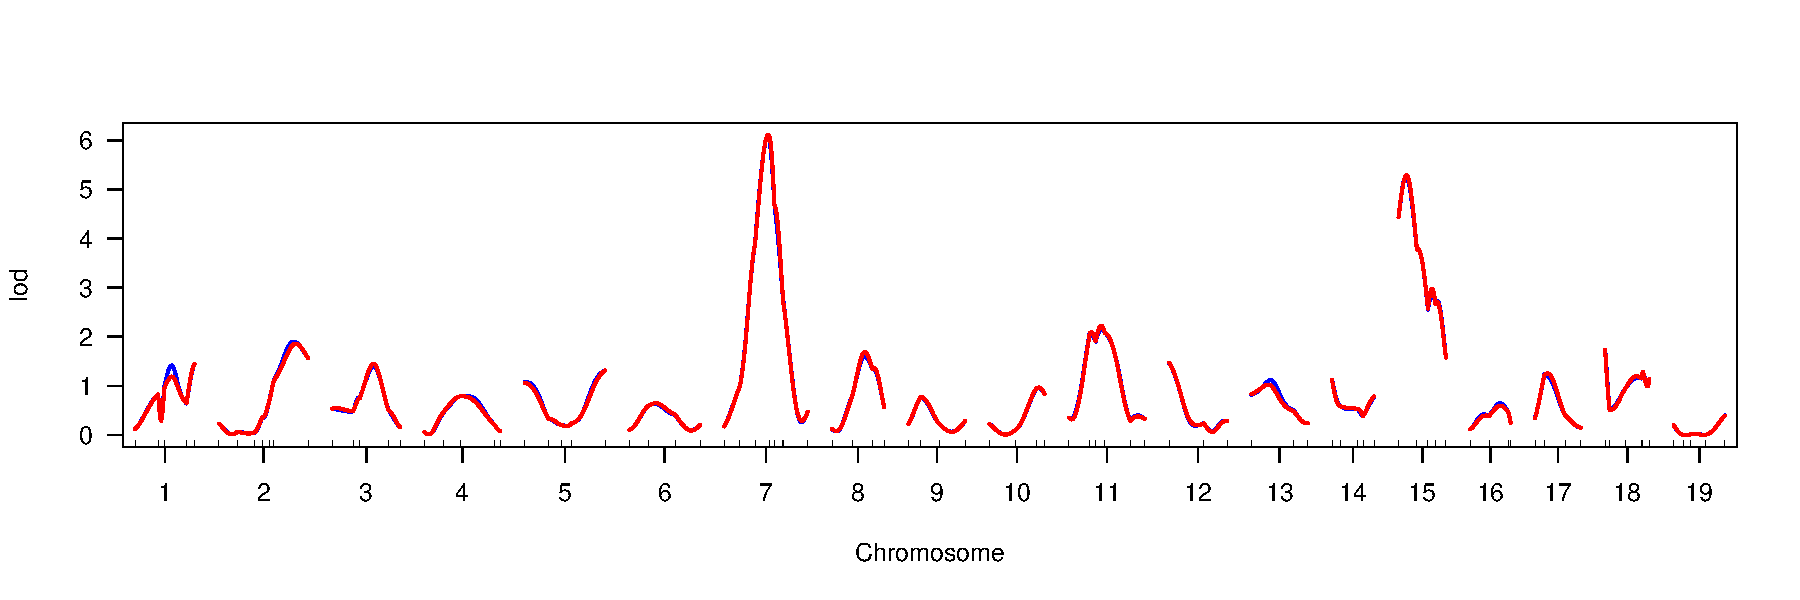
\includegraphics[width=\maxwidth]{RnwFigs/plot_em_and_hk-1} 

\end{knitrout}

Alternatively, we could do the following (figure not included, for brevity):

\begin{knitrout}
\definecolor{shadecolor}{rgb}{0.969, 0.969, 0.969}\color{fgcolor}\begin{kframe}
\begin{alltt}
\hlkwd{plot}\hlstd{(out.em,} \hlkwc{col}\hlstd{=}\hlstr{"blue"}\hlstd{)}
\hlkwd{plot}\hlstd{(out.hk,} \hlkwc{col}\hlstd{=}\hlstr{"red"}\hlstd{,} \hlkwc{add}\hlstd{=}\hlnum{TRUE}\hlstd{)}
\end{alltt}
\end{kframe}
\end{knitrout}

It's perhaps more informative to plot the differences:

\begin{knitrout}
\definecolor{shadecolor}{rgb}{0.969, 0.969, 0.969}\color{fgcolor}\begin{kframe}
\begin{alltt}
\hlkwd{plot}\hlstd{(out.hk} \hlopt{-} \hlstd{out.em,} \hlkwc{ylim}\hlstd{=}\hlkwd{c}\hlstd{(}\hlopt{-}\hlnum{0.3}\hlstd{,} \hlnum{0.3}\hlstd{),}
     \hlkwc{ylab}\hlstd{=}\hlstr{"LOD(HK)-LOD(EM)"}\hlstd{)}
\end{alltt}
\end{kframe}
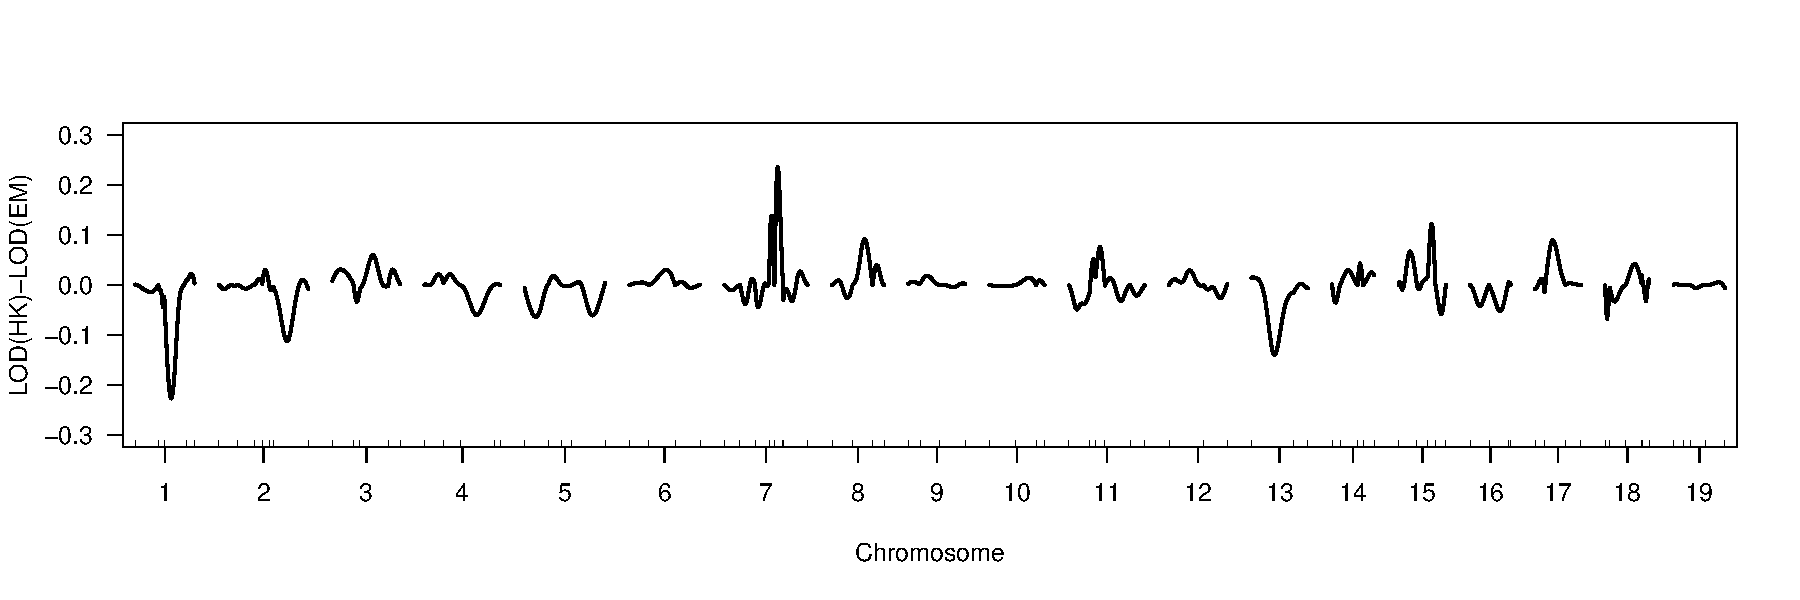
\includegraphics[width=\maxwidth]{RnwFigs/plot_diff-1} 

\end{knitrout}

\bigskip
{\sffamily \textbf{Permutation tests}}
\nopagebreak

To perform a permutation test, to get a genome-wide significance
threshold or genome-scan-adjusted p-values, we use {\tt scanone} just as
before, but with an additional argument, {\tt n.perm}, indicating the
number of permutation replicates.  It's quickest to use Haley-Knott
regression.

\begin{knitrout}
\definecolor{shadecolor}{rgb}{0.969, 0.969, 0.969}\color{fgcolor}\begin{kframe}
\begin{alltt}
\hlstd{operm} \hlkwb{<-} \hlkwd{scanone}\hlstd{(sug,} \hlkwc{method}\hlstd{=}\hlstr{"hk"}\hlstd{,} \hlkwc{n.perm}\hlstd{=}\hlnum{1000}\hlstd{)}
\end{alltt}
\begin{verbatim}
## Doing permutation in batch mode ...
\end{verbatim}
\end{kframe}
\end{knitrout}

A histogram of the results (the 1000 genome-wide maximum LOD
scores) is obtained as follows:

\begin{knitrout}
\definecolor{shadecolor}{rgb}{0.969, 0.969, 0.969}\color{fgcolor}\begin{kframe}
\begin{alltt}
\hlkwd{plot}\hlstd{(operm)}
\end{alltt}
\end{kframe}
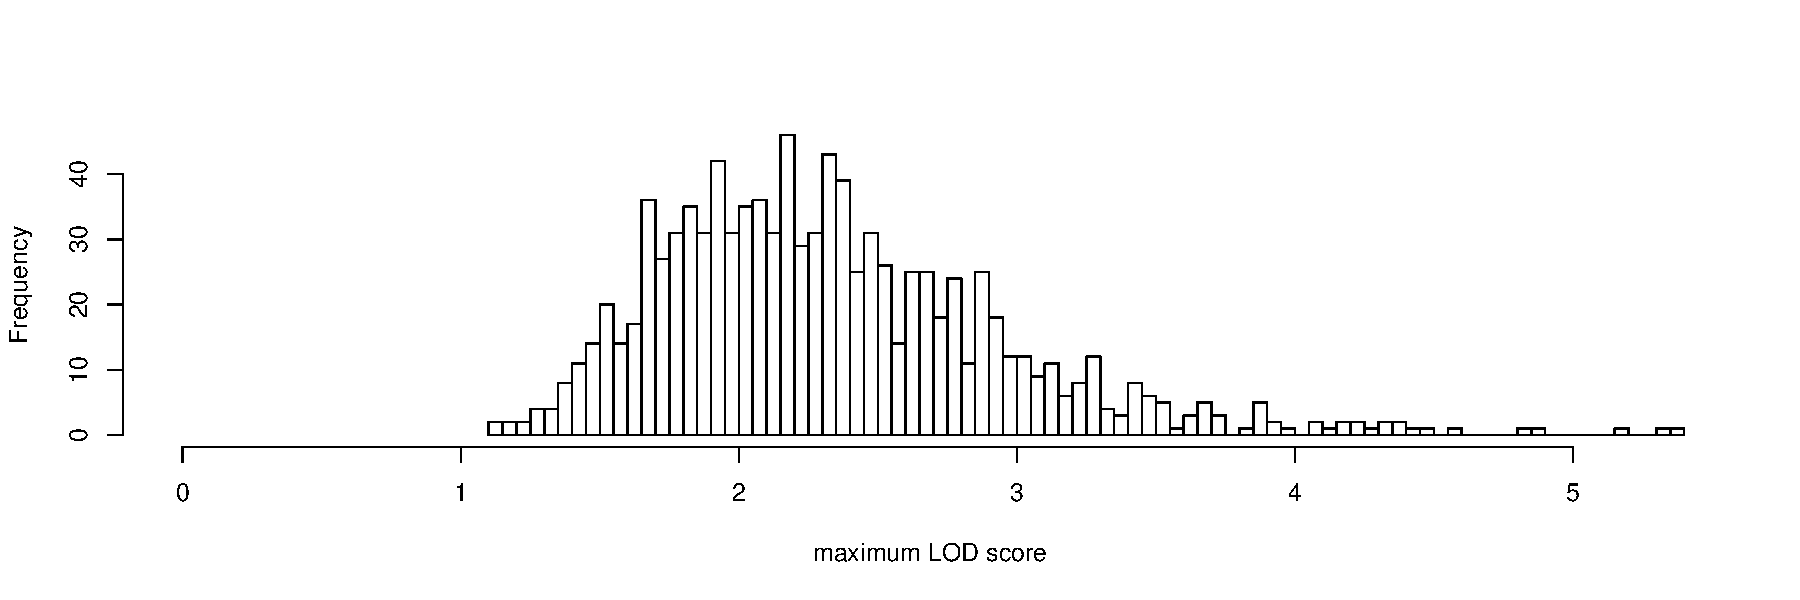
\includegraphics[width=\maxwidth]{RnwFigs/plot_perm-1} 

\end{knitrout}

Significance thresholds may be obtained via the {\tt summary}
function:

\begin{knitrout}
\definecolor{shadecolor}{rgb}{0.969, 0.969, 0.969}\color{fgcolor}\begin{kframe}
\begin{alltt}
\hlkwd{summary}\hlstd{(operm)}
\end{alltt}
\begin{verbatim}
## LOD thresholds (1000 permutations)
##      lod
## 5%  3.46
## 10% 3.12
\end{verbatim}
\begin{alltt}
\hlkwd{summary}\hlstd{(operm,} \hlkwc{alpha}\hlstd{=}\hlkwd{c}\hlstd{(}\hlnum{0.05}\hlstd{,} \hlnum{0.2}\hlstd{))}
\end{alltt}
\begin{verbatim}
## LOD thresholds (1000 permutations)
##      lod
## 5%  3.46
## 20% 2.78
\end{verbatim}
\end{kframe}
\end{knitrout}

The permutation results may be used along with
the {\tt scanone} results to have significance thresholds and
p-values calculated automatically:

\begin{knitrout}
\definecolor{shadecolor}{rgb}{0.969, 0.969, 0.969}\color{fgcolor}\begin{kframe}
\begin{alltt}
\hlkwd{summary}\hlstd{(out.hk,} \hlkwc{perms}\hlstd{=operm,} \hlkwc{alpha}\hlstd{=}\hlnum{0.2}\hlstd{,} \hlkwc{pvalues}\hlstd{=}\hlnum{TRUE}\hlstd{)}
\end{alltt}
\begin{verbatim}
##          chr  pos  lod  pval
## c7.loc45   7 47.7 6.11 0.000
## c15.loc8  15 12.0 5.29 0.002
\end{verbatim}
\end{kframe}
\end{knitrout}

\bigskip
{\sffamily \textbf{Interval estimates of QTL location}}
\nopagebreak

For the blood pressure phenotype, we've seen good evidence for QTL on
chromosomes 7 and 15.  Interval estimates of the location of QTL are
commonly obtained via 1.5-LOD support intervals, which may be
calculated via the function {\tt lodint}.  Alternatively, an
approximate Bayes credible interval may be obtained with
{\tt bayesint}.

To obtain the 1.5-LOD support interval and 95\% Bayes interval
for the QTL on chromosome 7, type the following.
The first and last rows define the ends of the intervals; the middle
row is the estimated QTL location.

\begin{knitrout}
\definecolor{shadecolor}{rgb}{0.969, 0.969, 0.969}\color{fgcolor}\begin{kframe}
\begin{alltt}
\hlkwd{lodint}\hlstd{(out.hk,} \hlkwc{chr}\hlstd{=}\hlnum{7}\hlstd{)}
\end{alltt}
\begin{verbatim}
##          chr   pos      lod
## c7.loc34   7 36.71 4.404165
## c7.loc45   7 47.71 6.107099
## c7.loc54   7 56.71 4.505278
\end{verbatim}
\begin{alltt}
\hlkwd{bayesint}\hlstd{(out.hk,} \hlkwc{chr}\hlstd{=}\hlnum{7}\hlstd{)}
\end{alltt}
\begin{verbatim}
##          chr   pos      lod
## c7.loc37   7 39.71 5.086176
## c7.loc45   7 47.71 6.107099
## c7.loc50   7 52.71 5.379287
\end{verbatim}
\end{kframe}
\end{knitrout}

It is sometimes useful to identify the closest flanking markers;
use {\tt expandtomarkers=TRUE}:

\begin{knitrout}
\definecolor{shadecolor}{rgb}{0.969, 0.969, 0.969}\color{fgcolor}\begin{kframe}
\begin{alltt}
\hlkwd{lodint}\hlstd{(out.hk,} \hlkwc{chr}\hlstd{=}\hlnum{7}\hlstd{,} \hlkwc{expandtomarkers}\hlstd{=}\hlnum{TRUE}\hlstd{)}
\end{alltt}
\begin{verbatim}
##          chr   pos      lod
## D7MIT176   7 34.48 3.894345
## c7.loc45   7 47.71 6.107099
## D7MIT7     7 63.14 2.800203
\end{verbatim}
\begin{alltt}
\hlkwd{bayesint}\hlstd{(out.hk,} \hlkwc{chr}\hlstd{=}\hlnum{7}\hlstd{,} \hlkwc{expandtomarkers}\hlstd{=}\hlnum{TRUE}\hlstd{)}
\end{alltt}
\begin{verbatim}
##          chr   pos      lod
## D7MIT176   7 34.48 3.894345
## c7.loc45   7 47.71 6.107099
## D7MIT323   7 54.45 4.690901
\end{verbatim}
\end{kframe}
\end{knitrout}

We can calculate the 2-LOD support interval and the 99\% Bayes
interval as follows.

\begin{knitrout}
\definecolor{shadecolor}{rgb}{0.969, 0.969, 0.969}\color{fgcolor}\begin{kframe}
\begin{alltt}
\hlkwd{lodint}\hlstd{(out.hk,} \hlkwc{chr}\hlstd{=}\hlnum{7}\hlstd{,} \hlkwc{drop}\hlstd{=}\hlnum{2}\hlstd{)}
\end{alltt}
\begin{verbatim}
##          chr   pos      lod
## c7.loc32   7 34.71 3.945848
## c7.loc45   7 47.71 6.107099
## c7.loc57   7 59.71 3.849972
\end{verbatim}
\begin{alltt}
\hlkwd{bayesint}\hlstd{(out.hk,} \hlkwc{chr}\hlstd{=}\hlnum{7}\hlstd{,} \hlkwc{prob}\hlstd{=}\hlnum{0.99}\hlstd{)}
\end{alltt}
\begin{verbatim}
##          chr   pos      lod
## c7.loc34   7 36.71 4.404165
## c7.loc45   7 47.71 6.107099
## c7.loc54   7 56.71 4.505278
\end{verbatim}
\end{kframe}
\end{knitrout}

The intervals for the chr 15 locus may be calculated as follows.

\begin{knitrout}
\definecolor{shadecolor}{rgb}{0.969, 0.969, 0.969}\color{fgcolor}\begin{kframe}
\begin{alltt}
\hlkwd{lodint}\hlstd{(out.hk,} \hlkwc{chr}\hlstd{=}\hlnum{15}\hlstd{)}
\end{alltt}
\begin{verbatim}
##           chr   pos      lod
## D15MIT175  15  3.96 4.432504
## c15.loc8   15 11.96 5.290136
## D15MIT184  15 22.82 3.778414
\end{verbatim}
\begin{alltt}
\hlkwd{bayesint}\hlstd{(out.hk,} \hlkwc{chr}\hlstd{=}\hlnum{15}\hlstd{)}
\end{alltt}
\begin{verbatim}
##           chr   pos      lod
## D15MIT175  15  3.96 4.432504
## c15.loc8   15 11.96 5.290136
## c15.loc16  15 19.96 4.373680
\end{verbatim}
\end{kframe}
\end{knitrout}


\bigskip
{\sffamily \textbf{R and package versions used}}
\nopagebreak

\begin{knitrout}
\definecolor{shadecolor}{rgb}{0.969, 0.969, 0.969}\color{fgcolor}\begin{kframe}
\begin{alltt}
\hlkwd{sessionInfo}\hlstd{()}
\end{alltt}
\begin{verbatim}
## R version 3.1.3 (2015-03-09)
## Platform: x86_64-w64-mingw32/x64 (64-bit)
## Running under: Windows 8 x64 (build 9200)
## 
## locale:
## [1] LC_COLLATE=English_United States.1252 
## [2] LC_CTYPE=English_United States.1252   
## [3] LC_MONETARY=English_United States.1252
## [4] LC_NUMERIC=C                          
## [5] LC_TIME=English_United States.1252    
## 
## attached base packages:
## [1] stats     graphics  grDevices utils     datasets 
## [6] methods   base     
## 
## other attached packages:
## [1] qtl_1.36-6 knitr_1.9 
## 
## loaded via a namespace (and not attached):
## [1] evaluate_0.5.5 formatR_1.1    highr_0.4.1   
## [4] parallel_3.1.3 stringr_0.6.2  tools_3.1.3
\end{verbatim}
\end{kframe}
\end{knitrout}

\end{document}
